\section{Entwicklung von Steuerungs- und eingebetteten Systemen}
Die technische Entwicklung von Steuerungs- und Regelungssystemen zeigt eine zunehmende Verlagerung von klassischen analogen Regelkreisen zu digitalen und vernetzten Systemarchitekturen (vgl. Abb.~\ref{fig:evolution_control_systems}).
Baillieul und Antsaklis beschreiben diesen Wandel als Übergang von klassischer Regelung über digitale Regelung hin zu vernetzten Regelungssystemen~\cite{baillieul2007networked}.
Diese Entwicklung ist für eingebettete Systeme relevant, da moderne Mikrocontroller lokale Datenverarbeitung mit digitaler Kommunikation verbinden können.

\begin{figure}[H]
    \centering
    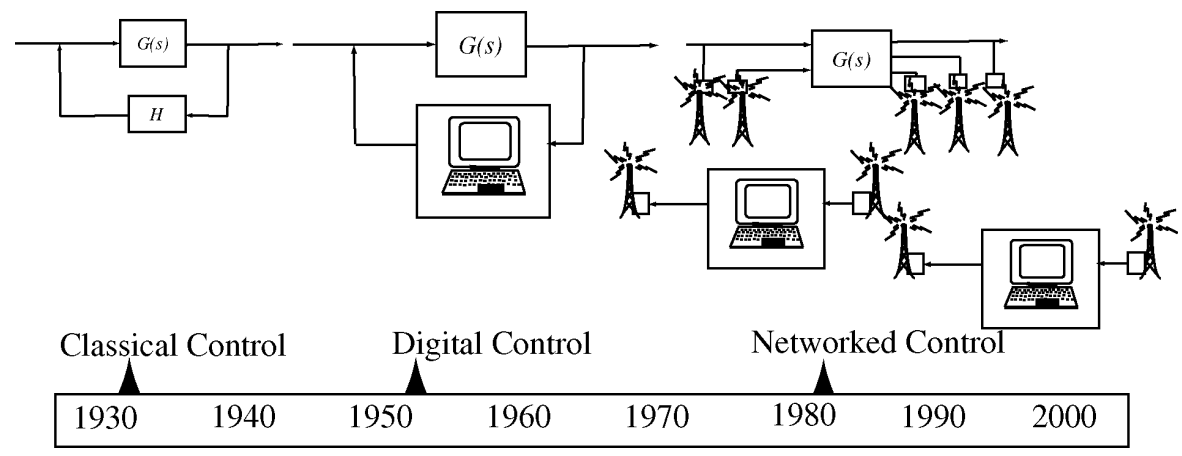
\includegraphics[width=0.85\textwidth]{inhalt/bilder/evolution_control_systems.png}
    \caption[Entwicklung von klassischer Regelung]{Entwicklung von klassischer Regelung über digitale Regelung hin zu vernetzten Systemen~\cite{baillieul2007networked}.}
    \label{fig:evolution_control_systems}
\end{figure}

Moderne Systeme zeichnen sich durch die Integration von Rechenleistung in dezentralen Komponenten sowie durch die Nutzung digitaler Kommunikationsnetze aus~\cite{baillieul2007networked}.
Dadurch können Daten lokal verarbeitet und gleichzeitig über Netzwerke ausgetauscht werden.
Diese Entwicklung bildet die Grundlage für Anwendungen im Bereich des \gls{iot}, bei denen eingebettete Systeme miteinander vernetzt sind.

Ein wesentliches Merkmal solcher Systeme ist das zeitliche Verhalten.
Kommunikationsverzögerungen, Paketverluste und schwankende Übertragungszeiten können die Systemfunktion beeinflussen~\cite{baillieul2007networked}.
Daher ist es erforderlich, zeitkritische Funktionen lokal auszuführen und externe Kommunikationsschnittstellen ergänzend einzusetzen.

Die entwickelte WordClock lässt sich in diese Entwicklung einordnen.
Sie kombiniert eine mikrocontrollerbasierte Steuerung mit netzwerkgestützten Funktionen, insbesondere zur Bereitstellung externer Zeitinformationen.
Damit stellt sie ein vernetztes eingebettetes System dar, bei dem lokale Verarbeitung und externe Kommunikation miteinander verknüpft sind.